\section{config.h File Reference}
\label{config_8h}\index{config.h@{config.h}}




This graph shows which files directly or indirectly include this file:\begin{figure}[H]
\begin{center}
\leavevmode
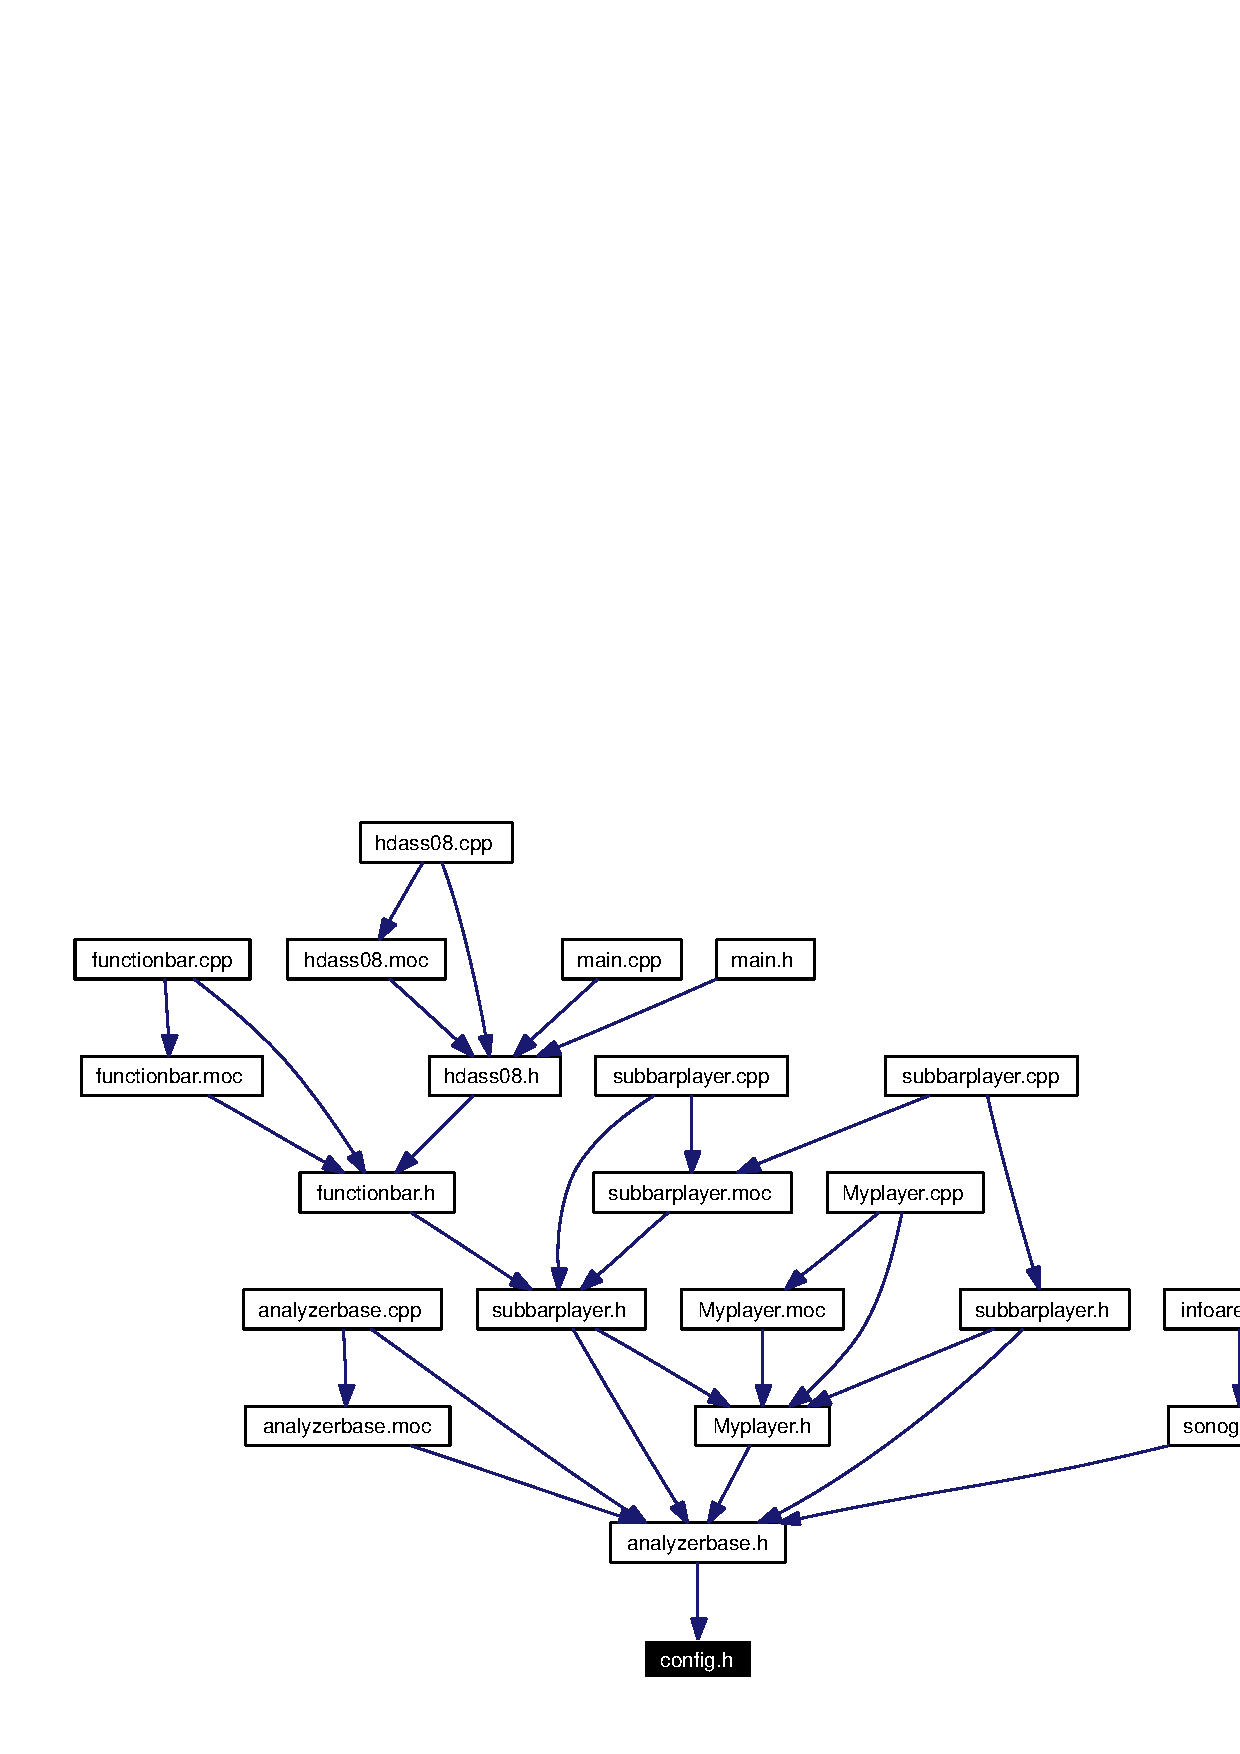
\includegraphics[width=365pt]{config_8h__dep__incl}
\end{center}
\end{figure}
\subsection*{Defines}
\begin{CompactItemize}
\item 
\#define {\bf HAVE\_\-CRYPT}\ 1
\item 
\#define {\bf HAVE\_\-DLFCN\_\-H}\ 1
\item 
\#define {\bf HAVE\_\-INTTYPES\_\-H}\ 1
\item 
\#define {\bf HAVE\_\-LIBJPEG}\ 1
\item 
\#define {\bf HAVE\_\-LIBPNG}\ 1
\item 
\#define {\bf HAVE\_\-LIBPTHREAD}\ 1
\item 
\#define {\bf HAVE\_\-LIBZ}\ 1
\item 
\#define {\bf HAVE\_\-MEMORY\_\-H}\ 1
\item 
\#define {\bf HAVE\_\-RES\_\-INIT}\ 1
\item 
\#define {\bf HAVE\_\-SGI\_\-STL}\ 1
\item 
\#define {\bf HAVE\_\-SNPRINTF}\ 1
\item 
\#define {\bf HAVE\_\-STDINT\_\-H}\ 1
\item 
\#define {\bf HAVE\_\-STDLIB\_\-H}\ 1
\item 
\#define {\bf HAVE\_\-STRINGS\_\-H}\ 1
\item 
\#define {\bf HAVE\_\-STRING\_\-H}\ 1
\item 
\#define {\bf HAVE\_\-SYS\_\-STAT\_\-H}\ 1
\item 
\#define {\bf HAVE\_\-SYS\_\-TYPES\_\-H}\ 1
\item 
\#define {\bf HAVE\_\-UNISTD\_\-H}\ 1
\item 
\#define {\bf HAVE\_\-VSNPRINTF}\ 1
\item 
\#define {\bf KDELIBSUFF}\ \char`\"{}\char`\"{}
\item 
\#define {\bf KDEMAXPATHLEN}\ 4096
\item 
\#define {\bf PACKAGE}\ \char`\"{}hdass08\char`\"{}
\item 
\#define {\bf PACKAGE\_\-BUGREPORT}\ \char`\"{}\char`\"{}
\item 
\#define {\bf PACKAGE\_\-NAME}\ \char`\"{}\char`\"{}
\item 
\#define {\bf PACKAGE\_\-STRING}\ \char`\"{}\char`\"{}
\item 
\#define {\bf PACKAGE\_\-TARNAME}\ \char`\"{}\char`\"{}
\item 
\#define {\bf PACKAGE\_\-VERSION}\ \char`\"{}\char`\"{}
\item 
\#define {\bf SIZEOF\_\-CHAR\_\-P}\ 4
\item 
\#define {\bf SIZEOF\_\-INT}\ 4
\item 
\#define {\bf SIZEOF\_\-LONG}\ 4
\item 
\#define {\bf SIZEOF\_\-SHORT}\ 2
\item 
\#define {\bf SIZEOF\_\-SIZE\_\-T}\ 4
\item 
\#define {\bf SIZEOF\_\-UNSIGNED\_\-LONG}\ 4
\item 
\#define {\bf STDC\_\-HEADERS}\ 1
\item 
\#define {\bf VERSION}\ \char`\"{}0.1\char`\"{}
\item 
\#define {\bf ksize\_\-t}\ socklen\_\-t
\end{CompactItemize}
\subsection*{Functions}
\begin{CompactItemize}
\item 
unsigned long {\bf strlcat} (char $\ast$, const char $\ast$, unsigned long)
\item 
unsigned long {\bf strlcpy} (char $\ast$, const char $\ast$, unsigned long)
\end{CompactItemize}


\subsection{Define Documentation}
\index{config.h@{config.h}!HAVE_CRYPT@{HAVE\_\-CRYPT}}
\index{HAVE_CRYPT@{HAVE\_\-CRYPT}!config.h@{config.h}}
\subsubsection{\setlength{\rightskip}{0pt plus 5cm}\#define HAVE\_\-CRYPT\ 1}\label{config_8h_a0}




Definition at line 11 of file config.h.\index{config.h@{config.h}!HAVE_DLFCN_H@{HAVE\_\-DLFCN\_\-H}}
\index{HAVE_DLFCN_H@{HAVE\_\-DLFCN\_\-H}!config.h@{config.h}}
\subsubsection{\setlength{\rightskip}{0pt plus 5cm}\#define HAVE\_\-DLFCN\_\-H\ 1}\label{config_8h_a1}




Definition at line 14 of file config.h.\index{config.h@{config.h}!HAVE_INTTYPES_H@{HAVE\_\-INTTYPES\_\-H}}
\index{HAVE_INTTYPES_H@{HAVE\_\-INTTYPES\_\-H}!config.h@{config.h}}
\subsubsection{\setlength{\rightskip}{0pt plus 5cm}\#define HAVE\_\-INTTYPES\_\-H\ 1}\label{config_8h_a2}




Definition at line 17 of file config.h.\index{config.h@{config.h}!HAVE_LIBJPEG@{HAVE\_\-LIBJPEG}}
\index{HAVE_LIBJPEG@{HAVE\_\-LIBJPEG}!config.h@{config.h}}
\subsubsection{\setlength{\rightskip}{0pt plus 5cm}\#define HAVE\_\-LIBJPEG\ 1}\label{config_8h_a3}




Definition at line 20 of file config.h.\index{config.h@{config.h}!HAVE_LIBPNG@{HAVE\_\-LIBPNG}}
\index{HAVE_LIBPNG@{HAVE\_\-LIBPNG}!config.h@{config.h}}
\subsubsection{\setlength{\rightskip}{0pt plus 5cm}\#define HAVE\_\-LIBPNG\ 1}\label{config_8h_a4}




Definition at line 23 of file config.h.\index{config.h@{config.h}!HAVE_LIBPTHREAD@{HAVE\_\-LIBPTHREAD}}
\index{HAVE_LIBPTHREAD@{HAVE\_\-LIBPTHREAD}!config.h@{config.h}}
\subsubsection{\setlength{\rightskip}{0pt plus 5cm}\#define HAVE\_\-LIBPTHREAD\ 1}\label{config_8h_a5}




Definition at line 26 of file config.h.\index{config.h@{config.h}!HAVE_LIBZ@{HAVE\_\-LIBZ}}
\index{HAVE_LIBZ@{HAVE\_\-LIBZ}!config.h@{config.h}}
\subsubsection{\setlength{\rightskip}{0pt plus 5cm}\#define HAVE\_\-LIBZ\ 1}\label{config_8h_a6}




Definition at line 29 of file config.h.\index{config.h@{config.h}!HAVE_MEMORY_H@{HAVE\_\-MEMORY\_\-H}}
\index{HAVE_MEMORY_H@{HAVE\_\-MEMORY\_\-H}!config.h@{config.h}}
\subsubsection{\setlength{\rightskip}{0pt plus 5cm}\#define HAVE\_\-MEMORY\_\-H\ 1}\label{config_8h_a7}




Definition at line 32 of file config.h.\index{config.h@{config.h}!HAVE_RES_INIT@{HAVE\_\-RES\_\-INIT}}
\index{HAVE_RES_INIT@{HAVE\_\-RES\_\-INIT}!config.h@{config.h}}
\subsubsection{\setlength{\rightskip}{0pt plus 5cm}\#define HAVE\_\-RES\_\-INIT\ 1}\label{config_8h_a8}




Definition at line 38 of file config.h.\index{config.h@{config.h}!HAVE_SGI_STL@{HAVE\_\-SGI\_\-STL}}
\index{HAVE_SGI_STL@{HAVE\_\-SGI\_\-STL}!config.h@{config.h}}
\subsubsection{\setlength{\rightskip}{0pt plus 5cm}\#define HAVE\_\-SGI\_\-STL\ 1}\label{config_8h_a9}




Definition at line 41 of file config.h.\index{config.h@{config.h}!HAVE_SNPRINTF@{HAVE\_\-SNPRINTF}}
\index{HAVE_SNPRINTF@{HAVE\_\-SNPRINTF}!config.h@{config.h}}
\subsubsection{\setlength{\rightskip}{0pt plus 5cm}\#define HAVE\_\-SNPRINTF\ 1}\label{config_8h_a10}




Definition at line 44 of file config.h.\index{config.h@{config.h}!HAVE_STDINT_H@{HAVE\_\-STDINT\_\-H}}
\index{HAVE_STDINT_H@{HAVE\_\-STDINT\_\-H}!config.h@{config.h}}
\subsubsection{\setlength{\rightskip}{0pt plus 5cm}\#define HAVE\_\-STDINT\_\-H\ 1}\label{config_8h_a11}




Definition at line 47 of file config.h.\index{config.h@{config.h}!HAVE_STDLIB_H@{HAVE\_\-STDLIB\_\-H}}
\index{HAVE_STDLIB_H@{HAVE\_\-STDLIB\_\-H}!config.h@{config.h}}
\subsubsection{\setlength{\rightskip}{0pt plus 5cm}\#define HAVE\_\-STDLIB\_\-H\ 1}\label{config_8h_a12}




Definition at line 50 of file config.h.\index{config.h@{config.h}!HAVE_STRING_H@{HAVE\_\-STRING\_\-H}}
\index{HAVE_STRING_H@{HAVE\_\-STRING\_\-H}!config.h@{config.h}}
\subsubsection{\setlength{\rightskip}{0pt plus 5cm}\#define HAVE\_\-STRING\_\-H\ 1}\label{config_8h_a14}




Definition at line 56 of file config.h.\index{config.h@{config.h}!HAVE_STRINGS_H@{HAVE\_\-STRINGS\_\-H}}
\index{HAVE_STRINGS_H@{HAVE\_\-STRINGS\_\-H}!config.h@{config.h}}
\subsubsection{\setlength{\rightskip}{0pt plus 5cm}\#define HAVE\_\-STRINGS\_\-H\ 1}\label{config_8h_a13}




Definition at line 53 of file config.h.\index{config.h@{config.h}!HAVE_SYS_STAT_H@{HAVE\_\-SYS\_\-STAT\_\-H}}
\index{HAVE_SYS_STAT_H@{HAVE\_\-SYS\_\-STAT\_\-H}!config.h@{config.h}}
\subsubsection{\setlength{\rightskip}{0pt plus 5cm}\#define HAVE\_\-SYS\_\-STAT\_\-H\ 1}\label{config_8h_a15}




Definition at line 71 of file config.h.\index{config.h@{config.h}!HAVE_SYS_TYPES_H@{HAVE\_\-SYS\_\-TYPES\_\-H}}
\index{HAVE_SYS_TYPES_H@{HAVE\_\-SYS\_\-TYPES\_\-H}!config.h@{config.h}}
\subsubsection{\setlength{\rightskip}{0pt plus 5cm}\#define HAVE\_\-SYS\_\-TYPES\_\-H\ 1}\label{config_8h_a16}




Definition at line 74 of file config.h.\index{config.h@{config.h}!HAVE_UNISTD_H@{HAVE\_\-UNISTD\_\-H}}
\index{HAVE_UNISTD_H@{HAVE\_\-UNISTD\_\-H}!config.h@{config.h}}
\subsubsection{\setlength{\rightskip}{0pt plus 5cm}\#define HAVE\_\-UNISTD\_\-H\ 1}\label{config_8h_a17}




Definition at line 77 of file config.h.\index{config.h@{config.h}!HAVE_VSNPRINTF@{HAVE\_\-VSNPRINTF}}
\index{HAVE_VSNPRINTF@{HAVE\_\-VSNPRINTF}!config.h@{config.h}}
\subsubsection{\setlength{\rightskip}{0pt plus 5cm}\#define HAVE\_\-VSNPRINTF\ 1}\label{config_8h_a18}




Definition at line 80 of file config.h.\index{config.h@{config.h}!KDELIBSUFF@{KDELIBSUFF}}
\index{KDELIBSUFF@{KDELIBSUFF}!config.h@{config.h}}
\subsubsection{\setlength{\rightskip}{0pt plus 5cm}\#define KDELIBSUFF\ \char`\"{}\char`\"{}}\label{config_8h_a19}




Definition at line 83 of file config.h.\index{config.h@{config.h}!KDEMAXPATHLEN@{KDEMAXPATHLEN}}
\index{KDEMAXPATHLEN@{KDEMAXPATHLEN}!config.h@{config.h}}
\subsubsection{\setlength{\rightskip}{0pt plus 5cm}\#define KDEMAXPATHLEN\ 4096}\label{config_8h_a20}




Definition at line 86 of file config.h.\index{config.h@{config.h}!ksize_t@{ksize\_\-t}}
\index{ksize_t@{ksize\_\-t}!config.h@{config.h}}
\subsubsection{\setlength{\rightskip}{0pt plus 5cm}\#define ksize\_\-t\ socklen\_\-t}\label{config_8h_a35}




Definition at line 217 of file config.h.\index{config.h@{config.h}!PACKAGE@{PACKAGE}}
\index{PACKAGE@{PACKAGE}!config.h@{config.h}}
\subsubsection{\setlength{\rightskip}{0pt plus 5cm}\#define PACKAGE\ \char`\"{}hdass08\char`\"{}}\label{config_8h_a21}




Definition at line 89 of file config.h.\index{config.h@{config.h}!PACKAGE_BUGREPORT@{PACKAGE\_\-BUGREPORT}}
\index{PACKAGE_BUGREPORT@{PACKAGE\_\-BUGREPORT}!config.h@{config.h}}
\subsubsection{\setlength{\rightskip}{0pt plus 5cm}\#define PACKAGE\_\-BUGREPORT\ \char`\"{}\char`\"{}}\label{config_8h_a22}




Definition at line 92 of file config.h.\index{config.h@{config.h}!PACKAGE_NAME@{PACKAGE\_\-NAME}}
\index{PACKAGE_NAME@{PACKAGE\_\-NAME}!config.h@{config.h}}
\subsubsection{\setlength{\rightskip}{0pt plus 5cm}\#define PACKAGE\_\-NAME\ \char`\"{}\char`\"{}}\label{config_8h_a23}




Definition at line 95 of file config.h.\index{config.h@{config.h}!PACKAGE_STRING@{PACKAGE\_\-STRING}}
\index{PACKAGE_STRING@{PACKAGE\_\-STRING}!config.h@{config.h}}
\subsubsection{\setlength{\rightskip}{0pt plus 5cm}\#define PACKAGE\_\-STRING\ \char`\"{}\char`\"{}}\label{config_8h_a24}




Definition at line 98 of file config.h.\index{config.h@{config.h}!PACKAGE_TARNAME@{PACKAGE\_\-TARNAME}}
\index{PACKAGE_TARNAME@{PACKAGE\_\-TARNAME}!config.h@{config.h}}
\subsubsection{\setlength{\rightskip}{0pt plus 5cm}\#define PACKAGE\_\-TARNAME\ \char`\"{}\char`\"{}}\label{config_8h_a25}




Definition at line 101 of file config.h.\index{config.h@{config.h}!PACKAGE_VERSION@{PACKAGE\_\-VERSION}}
\index{PACKAGE_VERSION@{PACKAGE\_\-VERSION}!config.h@{config.h}}
\subsubsection{\setlength{\rightskip}{0pt plus 5cm}\#define PACKAGE\_\-VERSION\ \char`\"{}\char`\"{}}\label{config_8h_a26}




Definition at line 104 of file config.h.\index{config.h@{config.h}!SIZEOF_CHAR_P@{SIZEOF\_\-CHAR\_\-P}}
\index{SIZEOF_CHAR_P@{SIZEOF\_\-CHAR\_\-P}!config.h@{config.h}}
\subsubsection{\setlength{\rightskip}{0pt plus 5cm}\#define SIZEOF\_\-CHAR\_\-P\ 4}\label{config_8h_a27}




Definition at line 107 of file config.h.\index{config.h@{config.h}!SIZEOF_INT@{SIZEOF\_\-INT}}
\index{SIZEOF_INT@{SIZEOF\_\-INT}!config.h@{config.h}}
\subsubsection{\setlength{\rightskip}{0pt plus 5cm}\#define SIZEOF\_\-INT\ 4}\label{config_8h_a28}




Definition at line 110 of file config.h.\index{config.h@{config.h}!SIZEOF_LONG@{SIZEOF\_\-LONG}}
\index{SIZEOF_LONG@{SIZEOF\_\-LONG}!config.h@{config.h}}
\subsubsection{\setlength{\rightskip}{0pt plus 5cm}\#define SIZEOF\_\-LONG\ 4}\label{config_8h_a29}




Definition at line 113 of file config.h.\index{config.h@{config.h}!SIZEOF_SHORT@{SIZEOF\_\-SHORT}}
\index{SIZEOF_SHORT@{SIZEOF\_\-SHORT}!config.h@{config.h}}
\subsubsection{\setlength{\rightskip}{0pt plus 5cm}\#define SIZEOF\_\-SHORT\ 2}\label{config_8h_a30}




Definition at line 116 of file config.h.\index{config.h@{config.h}!SIZEOF_SIZE_T@{SIZEOF\_\-SIZE\_\-T}}
\index{SIZEOF_SIZE_T@{SIZEOF\_\-SIZE\_\-T}!config.h@{config.h}}
\subsubsection{\setlength{\rightskip}{0pt plus 5cm}\#define SIZEOF\_\-SIZE\_\-T\ 4}\label{config_8h_a31}




Definition at line 119 of file config.h.\index{config.h@{config.h}!SIZEOF_UNSIGNED_LONG@{SIZEOF\_\-UNSIGNED\_\-LONG}}
\index{SIZEOF_UNSIGNED_LONG@{SIZEOF\_\-UNSIGNED\_\-LONG}!config.h@{config.h}}
\subsubsection{\setlength{\rightskip}{0pt plus 5cm}\#define SIZEOF\_\-UNSIGNED\_\-LONG\ 4}\label{config_8h_a32}




Definition at line 122 of file config.h.\index{config.h@{config.h}!STDC_HEADERS@{STDC\_\-HEADERS}}
\index{STDC_HEADERS@{STDC\_\-HEADERS}!config.h@{config.h}}
\subsubsection{\setlength{\rightskip}{0pt plus 5cm}\#define STDC\_\-HEADERS\ 1}\label{config_8h_a33}




Definition at line 125 of file config.h.\index{config.h@{config.h}!VERSION@{VERSION}}
\index{VERSION@{VERSION}!config.h@{config.h}}
\subsubsection{\setlength{\rightskip}{0pt plus 5cm}\#define VERSION\ \char`\"{}0.1\char`\"{}}\label{config_8h_a34}




Definition at line 128 of file config.h.

\subsection{Function Documentation}
\index{config.h@{config.h}!strlcat@{strlcat}}
\index{strlcat@{strlcat}!config.h@{config.h}}
\subsubsection{\setlength{\rightskip}{0pt plus 5cm}unsigned long strlcat (char $\ast$, const char $\ast$, unsigned {\em long})}\label{config_8h_a36}


\index{config.h@{config.h}!strlcpy@{strlcpy}}
\index{strlcpy@{strlcpy}!config.h@{config.h}}
\subsubsection{\setlength{\rightskip}{0pt plus 5cm}unsigned long strlcpy (char $\ast$, const char $\ast$, unsigned {\em long})}\label{config_8h_a37}


